\chapter{Foundation for Inference}
\label{FoundationForInference}

%_________________
%\section{Variability in Estimates}
%\label{VariabilityInEstimates}

%Figure~\ref{} shows the fraction of heads in 1, 2, 3, ..., 99,999, and 100,000 trials.
If we flip a fair coin 1,000 times and look at the fraction of heads, that proportion will be close to 0.5, but it probably won't be \emph{exactly} 0.5. If we flipped the coin many more times, the fraction would, on average, tend to get closer to 0.5. It may deviate at times away from 0.5, but those deviations will tend to get smaller and smaller with more data.

Studying this type of randomness is the focus of much of statistics. In this chapter, we'll explore this randomness in the context of several applications of statistics.

%_________________
\section{Case study: gender discrimination}
\label{caseStudyGenderDiscrimination}

\index{data!discrimination|(}

\begin{example}{Suppose your professor splits the students in class into two groups: students on the left and students on the right. If $\hat{p}_{_L}$ and $\hat{p}_{_R}$ represent the proportion of students who own an Apple product on the left and right, respectively, would you be surprised if $\hat{p}_{_L}$ did not {exactly} equal $\hat{p}_{_R}$?}\label{classRightLeftSideApple}
While the proportions would probably be close to each other, it would be unusual for them to be exactly the same. We would probably observe a small difference due to {chance}.
\end{example}

\begin{exercise}
If we don't think the side of the room a person sits on in class is related to whether the person owns an Apple product, what assumption are we making about the relationship between these two variables?\footnote{We would be assuming that these two variables are independent.}
\end{exercise}

\subsection{Variability within data}
\label{variabilityWithinData}

We consider a study investigating gender discrimination in the 1970s, which is set in the context of personnel decisions within a bank.\footnote{Rosen B and Jerdee T. 1974. Influence of sex role stereotypes on personnel decisions. Journal of Applied Psychology 59(1):9-14.} The research question we hope to answer~is, ``Are females discriminated against in promotion decisions made by male managers?"

The participants in this study are 48 male bank supervisors attending a management institute at the University of North Carolina in 1972. They were asked to assume the role of the personnel director of a bank and were given a personnel file to judge whether the person should be promoted to a branch manager position. The files given to the participants were identical, except that half of them indicated the candidate was male and the other half indicated the candidate was female. These files were randomly assigned to the subjects.

\begin{exercise}
Is this an observational study or an experiment? What implications does the study type have on what can be inferred from the results?\footnote{The study is an experiment, as subjects were randomly assigned a male file or a female file. Since this is an experiment, the results can be used to evaluate a causal relationship between gender of a candidate and the promotion decision.}
\end{exercise}

For each supervisor we record the gender associated with the assigned file and the promotion decision. Using the results of the study summarized in Table~\ref{discriminationResults}, we would like to evaluate if females are unfairly discriminated against in promotion decisions. In this study, a smaller proportion of females are promoted than males (0.583 versus 0.875), but it is unclear whether the difference provides \emph{convincing evidence} that females are unfairly discriminated against.

\begin{table}[ht]
\centering
\begin{tabular}{l l cc rr}
& & \multicolumn{2}{c}{\var{decision}} \\
  \cline{3-4}
		&			& 	{promoted} 	& {not promoted} & Total & \hspace{3mm}  \\ 
  \cline{2-5}
		&	{male} 			& 21    		& 3   & 24  	 \\ 
  \raisebox{1.5ex}[0pt]{\var{gender}}		&	{female} 	& 14    		& 10     & 24	 \\ 
  \cline{2-5}
  		&	Total		& 35	& 13	&  48 \\
  \cline{2-5}
\end{tabular}
\caption{Summary results for the gender discrimination study.}
\label{discriminationResults}
\end{table}

\begin{example}{Statisticians are sometimes called upon to evaluate the strength of evidence. When looking at the rates of promotion for males and females in this study, what comes to mind as we try to determine whether the data show convincing evidence of a real difference?} \label{discriminationResultsWhatIsConvincingEvidence}
The observed promotion rates (58.3\% for females versus 87.5\% for males) suggest there might be discrimination against women in promotion decisions. However, we cannot be sure if the observed difference represents discrimination or is just from random chance. Generally there is a little bit of fluctuation in sample data, and we wouldn't expect the sample proportions to be \emph{exactly} equal, even if the truth was that the promotion decisions were independent of gender.
\end{example}

Example~\ref{discriminationResultsWhatIsConvincingEvidence} is a reminder that the observed outcomes in the sample may not perfectly reflect the true relationships between variables in the underlying population. Table~\ref{discriminationResults} shows there were 7 fewer promotions in the female group than in the male group, a difference in promotion rates of 29.2\% $\left( \frac{21}{24} - \frac{14}{24} = 0.292 \right)$. This difference is large, but the sample size for the study is small, making it unclear if this observed difference represents discrimination or whether it is simply due to chance. We label these two competing claims, $H_0$ and $H_A$:
\begin{itemize}
\setlength{\itemsep}{0mm}
\item[$H_0$:] \textbf{Independence model.} The variables \var{gender} and \var{decision} are independent. They have no relationship, and the observed difference between the proportion of males and females who were promoted, 29.2\%, was due to chance.
\item[$H_A$:] \textbf{Alternative model.} The variables \var{gender} and \var{decision} are \emph{not} independent. The difference in promotion rates of 29.2\% was not due to chance, and equally qualified females are less likely to be promoted than males.
\end{itemize}

What would it mean if the independence model, which says the variables \var{gender} and \var{decision} are unrelated, is true? It would mean each banker was going to decide whether to promote the candidate without regard to the gender indicated on the file. That~is, the difference in the promotion percentages was due to the way the files were randomly divided to the bankers, and the randomization just happened to give rise to a relatively large difference of 29.2\%.

Consider the alternative model: bankers were influenced by which gender was listed on the personnel file. If this was true, and especially if this influence was substantial, we would expect to see some difference in the promotion rates of male and female candidates. If this gender bias was against females, we would expect a smaller fraction of promotion decisions for female personnel files relative to the male files.

We choose between these two competing claims by assessing if the data conflict so much with $H_0$ that the independence model cannot be deemed reasonable. If this is the case, and the data support $H_A$, then we will reject the notion of independence and conclude there was discrimination.

\subsection{Simulating the study}
\label{simulatingTheStudy}

Table~\ref{discriminationResults} shows that 35 bank supervisors recommended promotion and 13 did not. Now, suppose the banker's decisions were independent of gender. Then, if we conducted the experiment again with a different random arrangement of files, differences in promotion rates would be based only on random fluctuation. We can actually perform this \term{randomization}, which simulates what would have happened if the bankers decisions had been independent of gender but we had distributed the files differently.

In this \term{simulation}, we thoroughly shuffle 48 personnel files, 24 labeled \resp{male\_\hspace{0.3mm}sim} and 24 labeled \resp{female\_\hspace{0.3mm}sim}, and deal these files into two stacks. We will deal 35 files into the first stack, which will represent the 35 supervisors who recommended promotion. The second stack will have 13 files, and it will represent the 13 supervisors who recommended against promotion. Then, as we did with the original data, we tabulate the results and determine the fraction of \resp{male\_\hspace{0.3mm}sim} and \resp{female\_\hspace{0.3mm}sim} who were promoted. The randomization of files in this simulation is independent of the promotion decisions, which means any difference in the two fractions is entirely due to chance. Table~\ref{discriminationRand1} show the results of such a simulation.

\begin{table}[ht]
\centering
\begin{tabular}{l l cc rr}
& & \multicolumn{2}{c}{\var{decision}} \\
  \cline{3-4}
		&			& 	{promoted} 	& {not promoted} & Total & \hspace{3mm}  \\ 
  \cline{2-5}
		&	\resp{male\_\hspace{0.3mm}sim} 					& 18    		& 6    & 24 	 \\ 
  \raisebox{1.5ex}[0pt]{\var{gender\_\hspace{0.3mm}sim}}		&	\resp{female\_\hspace{0.3mm}sim} 	& 17    		& 7 & 24    	 \\ 
  \cline{2-5}
  & Total	& 35 & 13 & 48
\end{tabular}
\caption{Simulation results, where any difference in promotion rates between \resp{male\_\hspace{0.3mm}sim} and \resp{female\_\hspace{0.3mm}sim} is purely due to chance.}
\label{discriminationRand1}
\end{table}

\begin{exercise} \label{sampleDifferenceInMaleAndFemaleDiscrimination}
What is the difference in promotion rates between the two simulated groups in Table~\ref{discriminationRand1}? How does this compare to the observed 29.2\% in the actual groups?\footnote{$18/24 - 17/24=0.042$ or about 4.2\% in favor of the men. This difference due to chance is much smaller than the difference observed in the actual groups.}
\end{exercise}

\textB{\pagebreak}

\subsection{Checking for independence}

We computed one possible difference under the independence model in Exercise~\ref{sampleDifferenceInMaleAndFemaleDiscrimination}, which represents one difference due to chance. While in this first simulation, we physically dealt out files, it is more efficient to perform this simulation using a computer. Repeating the simulation on a computer, we get another difference due to chance: -0.042. And another: 0.208. And so on until we repeat the simulation enough times that we have a good idea of what represents the \emph{distribution of differences from chance alone}. Figure~\ref{discRandDotPlot} shows a plot of the differences found from 100 simulations, where each dot represents a simulated difference between the proportions of male and female files that were recommended for promotion.

\begin{figure}[ht]
\centering
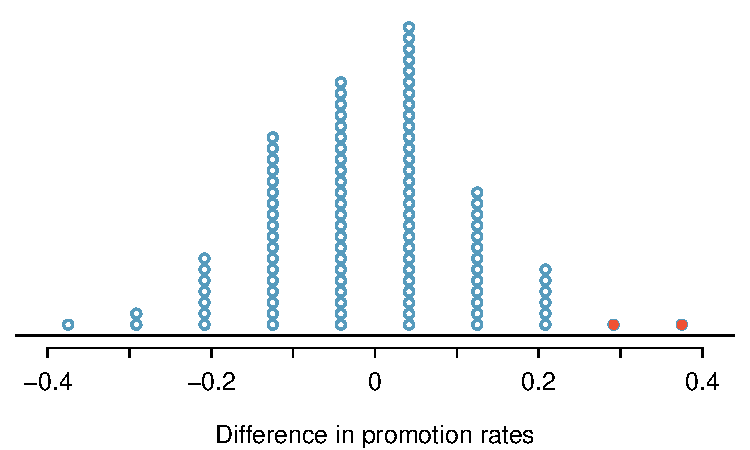
\includegraphics[width=0.7\textwidth]{02/figures/discRandDotPlot/discRandDotPlot}
\caption{A stacked dot plot of differences from 100 simulations produced under the independence model, $H_0$, where \var{gender\_\hspace{0.3mm}sim} and \var{decision} are independent. Two of the 100 simulations had a difference of at least 29.2\%, the difference observed in the study.}
\label{discRandDotPlot}
\end{figure}

Note that the distribution of these simulated differences is centered around 0. We simulated these differences assuming that the independence model was true, and under this condition, we expect the difference to be zero with some random fluctation. We would generally be surprised to see a difference of \emph{exactly} 0: sometimes, just by chance, the difference is higher than 0, and other times it is lower than zero.

\begin{example}{How often would you observe a difference of at least 29.2\% (0.292) according to Figure~\ref{discRandDotPlot}? Often, sometimes, rarely, or never?}
It appears that a difference of at least 29.2\% due to chance alone would only happen about 2\% of the time according to Figure~\ref{discRandDotPlot}. Such a low probability indicates a rare event.
\end{example}

The difference of 29.2\% being a rare event suggests two possible interpretations of the results of the study:
\begin{itemize}
\setlength{\itemsep}{0mm}
\item[$H_0$] \textbf{Independence model.} Gender has no effect on promotion decision, and we observed a difference that would only happen rarely.
\item[$H_A$] \textbf{Alternative model.} Gender has an effect on promotion decision, and what we observed was actually due to equally qualified women being discriminated against in promotion decisions, which explains the large difference of 29.2\%.
\end{itemize}
Based on the simulations, we have two options. (1)~We conclude that the study results do not provide strong evidence against the independence model. That is, we do not have sufficiently strong evidence to conclude there was gender discrimination. (2)~We conclude the evidence is sufficiently strong to reject $H_0$ and assert that there was gender discrimination. When we conduct formal studies, usually we reject the notion that we just happened to observe a rare event.\footnote{This reasoning does not generally extend to anecdotal observations. Each of us observes incredibly rare events every day, events we could not possibly hope to predict. However, in the non-rigorous setting of anecdotal evidence, almost anything may appear to be a rare event, so the idea of looking for rare events in day-to-day activities is treacherous. For example, we might look at the lottery: there was only a 1 in 176 million chance that the Mega Millions numbers for the largest jackpot in history (March 30, 2012) would be (2, 4, 23, 38, 46) with a Mega ball of (23), but nonetheless those numbers came up! However, no matter what numbers had turned up, they would have had the same incredibly rare odds. That is, \emph{any set of numbers we could have observed would ultimately be incredibly rare}. This type of situation is typical of our daily lives: each possible event in itself seems incredibly rare, but if we consider every alternative, those outcomes are also incredibly rare. We should be cautious not to misinterpret such anecdotal evidence.} So in this case, we reject the independence model in favor of the alternative. That is, we are concluding the data provide strong evidence of gender discrimination against women by the supervisors.

\index{data!discrimination|)}

One field of statistics, statistical inference, is built on evaluating whether such differences are due to chance. In statistical inference, statisticians evaluate which model is most reasonable given the data. Errors do occur, just like rare events, and we might choose the wrong model. While we do not always choose correctly, statistical inference gives us tools to control and evaluate how often these errors occur. In Chapter~\ref{foundationsForInference}, we give a formal introduction to the problem of model selection. We spend the next two chapters building a foundation of probability and theory necessary to make that discussion rigorous.


%_________________
%\section{Case study: stents and strokes [2 prop randomization]}

%_________________
\section{Case study: opportunity cost}

How rational and consistent is the behavior of the typical American college student? In this section, we'll explore whether consumers always consider an obvious fact: money not spent now can be spent later.

In particular, we are interested whether reminding students about this well-known fact about money causes them to be a little more thrifty. A skeptic might think that such a reminder would have no impact. We can summarize these two perspectives using the null and alternative hypothesis framework.
\begin{itemize}
\setlength{\itemsep}{0mm}
\item[$H_0$:] \textbf{Independence model.} Reminding students that they can save money for later purchases will not have any impact on students' spending decisions.
\item[$H_A$:] \textbf{Alternative model.} Reminding students that they can save money for later purchases will reduce the chance that they will continue with a purchase.
\end{itemize}
In this section, we'll explore an experiment conducted by five researchers that investigates this very question for students at a southwestern university in the United States.\footnote{Frederick S, Novemsky N, Wang J, Dhar R, Nowlis S. 2009. Opportunity Cost Neglect. Journal of Consumer Research 36: 553-561.}

\subsection{Opportunity costs and consumer choice data}

%Shane Frederick of Yale School of Management and his collaborators conducted an experiment exploring the rational behavior of consumers. 
One-hundred and fifty students were recruited for the study from a southwestern university, and each was given the following statement:
\begin{quote}
Suppose when a person is about to spend money, we simply reminded them that they could spend the money on something else. Would it have any impact on the likelihood that they would continue with the purchase?

What would you do in this situation? Please circle one of the options below.
\end{quote}
Half of the 150 students were randomized into a control group and were given the following two options:
\begin{quote}
(A) Buy this entertaining video.

(B) Not buy this entertaining video.
\end{quote}
The remaining 75 students were placed in the treatment group, and they saw a slightly different option (B):
\begin{quote}
(A) Buy this entertaining video.

(B) Not buy this entertaining video. Keep the \$14.99 for other purchases.
\end{quote}
Would the extra statement reminding students that if they don't spend money now they could spend it later have an impact on the decision they would make? Table~\ref{OpportunityCostTable} summarizes the study results.

\begin{table}[ht]
\centering
\begin{tabular}{l cc rr}
& \multicolumn{2}{c}{decision} \\
\cline{2-3}
				& {buy DVD}\ \  	& {not buy DVD} & Total & \hspace{3mm}  \\ 
\cline{1-4}
control group 		& 56		& 19	& 75 \\ 
treatment group 	& 41		& 34	& 75 \\ 
\cline{1-4}
Total				& 97		& 53	& 150
\end{tabular}
\caption{Summary of student choices in the opportunity cost study.}
%150 participants were asked whether they would buy a DVD under a particular circumstance. Participants in the control group were given two options, and participants in the treatment group were given the same options, except in the \emph{not buy} option they were reminded that not spending the money meant the money could be used for a later purchase. This table summarizes the results from the study.}
\label{OpportunityCostTable}
\end{table}

It might be a little easier to review the results using row proportions, where it would be easier to review the proportion of participants in each group who said they would buy or not buy the DVD. These summaries are given in Table~\ref{OpportunityCostTableRowProp}.

\begin{table}[ht]
\centering
\begin{tabular}{l cc rr}
& \multicolumn{2}{c}{decision} \\
\cline{2-3}
				& {buy DVD}\ \  	& {not buy DVD} & Total & \hspace{3mm}  \\ 
\cline{1-4}
control group 		& 0.747	& 0.253	& 1.000 \\ 
treatment group 	& 0.547	& 0.453	& 1.000 \\ 
\cline{1-4}
Total				& 0.647	& 0.353	& 1.000
\end{tabular}
\caption{Table~\ref{OpportunityCostTable} summarized using row proportions.}
\label{OpportunityCostTableRowProp}
\end{table}

A first look at the data suggests that reminding students that not spending money means they can spend the money later has an impact. The difference in the proportion of students who did not buy the DVD was 20\% higher in the treatment group than in the control group:
\begin{align*}
\hat{p}_{trmt} - \hat{p}_{ctrl}
  = \frac{34}{75} - \frac{19}{75}
  = 0.453 - 0.253
  = 0.200
\end{align*}
However, is this result \term{statistically significant}? That is, is a 20\% difference so prominent that it is unlikely it would occur from chance alone?

\subsection{Results from chance alone}

The primary goal in this data analysis will be to understand what sort of differences we might see if the treatment had no effect on students. For this, we'll use randomization.

Suppose the treatment had no impact on student decisions. In that case, the difference between the groups was by chance -- a result of the way students were randomized into groups. We can repeat this randomization under the scenario where there is no treatment effect.

We'll take the students and randomize them into two new groups, fake-control and fake-treatment, and then we'll look at the difference in the two groups. The results of this new randomization are shown in Table~\ref{OpportunityCostTableFake}. From this table, we can compute the difference in the proportions of students who would or would not buy the DVD:
\begin{align*}
\hat{p}_{trmt} - \hat{p}_{ctrl}
  = \frac{24}{75} - \frac{29}{75}
  = 0.32 - 0.387
  = - 0.067
\end{align*}
This difference of -6.7\% is entirely due to chance.

\begin{table}[ht]
\centering
\begin{tabular}{l cc rr}
& \multicolumn{2}{c}{decision} \\
\cline{2-3}
				& {buy DVD}\ \  	& {not buy DVD} & Total & \hspace{3mm}  \\ 
\cline{1-4}
\textbf{fake}-control group 		& 46		& 29	& 75 \\ 
\textbf{fake}-treatment group 	& 51		& 24	& 75 \\ 
\cline{1-4}
Total				& 97		& 53	& 150
\end{tabular}
\caption{Summary of student choices against their fake groups. The group assignment had no connection to the student decisions, so any difference between the two groups is due to chance.}
\label{OpportunityCostTableFake}
\end{table}

It will be helpful to get a more complete sense of what sorts of differences would happen from chance alone. To find out, we'll simulate another set of fake groups and compute the new difference: 0.013. And again: 0.067. And again: -0.173. We'll do this 10,000 times. The results are summarized in a histogram in Figure~\ref{OpportunityCostDotPlot}, where the height of each histogram bar represents the fraction of observations in that group.

\begin{figure}[ht]
\centering
\includegraphics[width=0.8\textwidth]{02/figures/OpportunityCost/OpportunityCostDotPlot}
\caption{A histogram of 5,000 chance differences produced under the independence model, $H_0$. 1.1\% of the simulations had a difference of at least 20\%, which was the difference observed in the study.}
\label{OpportunityCostDotPlot}
\end{figure}

If there was no treatment effect, then we'd only observe a difference of at least +20\% about 0.35\% of the time, or about 1 in 300 times. That is really rare! Instead, we will conclude that the data provide strong evidence that there is a treatment effect: reminding students before a purchase that they could instead spend the money on something else later lowers the chance that they will continue with the purchase.



% conducted the study again with the same students. If the treatment had no influence on their decisions, each student would respond the same. We would still have 97 students would would buy the DVD and 53 students who would not. If we randomly split these students up into the treatment and control groups, we are simulating what might have happened if (1) we could repeat the study and (2) the null hypothesis was true, meaning the treatment has no effect.

%Table~\ref{} represents a new randomization of students into the treatment and control groups. In this simulation, we see that the 




%What if we could encourage more thoughtful spending by consumers by pointing out the obvious fact that they could spend money on different things? This was the 
%
%Capitalism is built on the premise that individuals make rational decision. What if we could 
%
%What if we told you there was a simple way to make people more thoughtful about how they spend their money?
%
%If shoppers are reminded that if they don't spend money today, they can spend it tomorrow, do you think that would have an influence on their shopping behavior?
%
%Consider the following scenario, which was given to 150 students:
%\begin{quote}
%Imagine that you have been saving some extra money on the side to make some purchases, and on your most recent visit to the video store you come across a special sale on a new video. This video is one with your favorite actor or actress, and your favorite type of movie (such as a comedy, drama, thriller, etc.). This particular video that you are considering is one you have been thinking about buying for a long time. It is available for a special sale price of \$14.99.
%\end{quote}





%_________________
\section{Hypothesis testing}

In the last two sections, we utilized a \term{hypothesis test}, which is a formal technique for evaluating two competing possibilities. In each scenario, we described a \term{null hypothesis}, which typically represents either a skeptical perspective or a perspective of no difference. We also laid out an \term{alternative hypothesis}, which often represented a new perspective, such as the possibility that there has been a change.

\begin{termBox}{\tBoxTitle{Null and alternative hypotheses}
{\small The \term{null hypothesis ($H_0$)} often represents either a skeptical perspective or a claim to be tested. The \term{alternative hypothesis ($H_A$)} represents an alternative claim under consideration and is often represented by a range of possible parameter values.}}
\end{termBox}

The hypothesis testing framework is a very general tool, and we often use it without a second thought. If a person makes a somewhat unbelievable claim, we are initially skeptical. However, if there is sufficient evidence that supports the claim, we set aside our skepticism and reject the null hypothesis in favor of the alternative. The hallmarks of hypothesis testing are also found in the US court system. 

\subsection{Hypothesis testing in the US court system}

\begin{exercise} \label{hypTestCourtExample}
A US court considers two possible claims about a defendant: she is either innocent or guilty. If we set these claims up in a hypothesis framework, which would be the null hypothesis and which the alternative?\footnote{The jury considers whether the evidence is so convincing (strong) that there is no reasonable doubt regarding the person's guilt. That is, the skeptical perspective is that the person is innocent (null hypothesis) until evidence is presented that convinces the jury that the person is guilty (alternative hypothesis).}
\end{exercise}

Jurors examine the evidence to see whether it convincingly shows a defendant is guilty. Even if the jurors leave unconvinced of guilt beyond a reasonable doubt, this does not mean they believe the defendant is innocent. This is also the case with hypothesis testing: \emph{even if we fail to reject the null hypothesis, we typically do not accept the null hypothesis as true}. Failing to find strong evidence for the alternative hypothesis is not equivalent to accepting the null hypothesis or proving that it is true.

%\begin{tipBox}{\tipBoxTitle{We never accept the null hypothesis}
%Statistics trains us to keep an }
%\end{tipBox}

\subsection{Revisiting the gender discrimination case study}

In Section~\ref{caseStudyGenderDiscrimination} we encountered a study from the 1970's that explored whether there was strong evidence that women were less likely to be promoted than men.

In this study, we framed our investigation into four pieces:
\begin{enumerate}
\item \textbf{Frame the research question and construct hypotheses.} Are females discriminated against in promotion decisions made by male managers? More formally, we constructed hypotheses:
\begin{itemize}
\item[$H_0$] Gender has no effect on promotion decision.
\item[$H_A$] Gender has some effect on promotion decision.
\end{itemize}
The null hypothesis ($H_0$) was a perspective of no difference.
\item \textbf{Collect relevant data.} Researches conducted an experiment with 48 male bank supervisors. Half of the supervisors received a personnel file for a woman and the other half received a personnel file that was identical, except that the candidate was listed as a man. The summary table may be found on page~\pageref{discriminationResults}.
\item \textbf{Analyze the data.} We found that the recommended promotion rate was 29.2\% lower for women. From a skeptical perspective, we asked whether this difference could be due to chance. To test this idea, we constructed differences that were actually due to chance, and we determined that if there was no discrimination, then we got what are very unlikely results: we would only observe such a large difference from chance alone about 2\% of the time!
\item \textbf{Form a conclusion.} The data indicated that it was very unlikely to see such a large difference from chance alone. For this reason, we would reject the null hypothesis and conclude there was discrimination in the study
\end{enumerate}
% the skeptical perspective was one of \emph{no difference}: the promotion rates were the same among men and women.


\subsection{Revisiting the opportunity cost case study}


\subsection{Hypothesis testing framework}


%_________________
\section{Decision Errors}


%_________________
\section{Case study: tappers and listeners [1 prop simulation]}


%_________________
\section{Case study: surviving a recession [1 prop simulation]}


%_________________
\section{Confidence intervals}

